\documentclass[12pt]{article}
\usepackage[english]{babel}
\usepackage[utf8]{inputenc}

%% Pointer to 'default' preamble
% pacakages and definitions

\usepackage{geometry}
\geometry{
	letterpaper, 
	portrait, 
	top=.75in,
	left=.8in,
	right=.75in,
	bottom=.5in		} 	% Page Margins
	
%% additional packages for nice things
\usepackage{amsmath} 	% for most math
\usepackage{commath} 	% for abs
\usepackage{lastpage}	% for page count
\usepackage{amssymb} 	% for therefore
\usepackage{graphicx} 	% for image handling
\usepackage{wrapfig} 	% wrap figures
\usepackage[none]{hyphenat} % for no hyphenations
\usepackage{array} 		% for >{} column characterisctis
\usepackage{physics} 	% for easier derivative \dv....
\usepackage{tikz} 		% for graphic@!
\usepackage{circuitikz} % for circuits!
\usetikzlibrary{arrows.meta} % for loads
\usepackage[thicklines]{cancel}	% for cancels
\usepackage{xcolor}		% for color cancels
\usepackage[per-mode=fraction]{siunitx} % for si units and num
\sisetup{group-separator = {,}, group-minimum-digits = 3} % additional si unit table functionality

\usepackage{fancyhdr} 	% for header
\usepackage{comment}	% for ability to comment out large sections
\usepackage{multicol}	% for multiple columns using multicols
\usepackage[framed,numbered]{matlab-prettifier} % matlab sytle listing
\usepackage{marvosym} 	% for boltsymbol lightning
\usepackage{pdflscape} 	% for various landscape pages in portrait docs.
%\usepackage{float}
\usepackage{fancyvrb}	% for Verbatim (a tab respecting verbatim)
\usepackage{enumitem}	% for [resume] functionality of enumerate
\usepackage{spreadtab} 	% for using formulas in tables}
\usepackage{numprint}	% for number format in spread tab
\usepackage{subcaption} % for subfigures with captions
\usepackage[normalem]{ulem} % for strike through sout

% for row colors in tables....
\usepackage{color, colortbl}
\definecolor{G1}{gray}{0.9}
\definecolor{G2}{rgb}{1,0.88,1}%{gray}{0.6}
\definecolor{G3}{rgb}{0.88,1,1}

% For table formatting
\usepackage{booktabs}
\renewcommand{\arraystretch}{1.2}
\usepackage{floatrow}
\floatsetup[table]{capposition=top} % put table captions on top of tables

% Caption formating footnotesize ~ 10 pt in a 12 pt document
\usepackage[font={small}]{caption}

%% package config 
\sisetup{output-exponent-marker=\ensuremath{\mathrm{E}}} % for engineer E
\renewcommand{\CancelColor}{\color{red}}	% for color cancels
\lstset{aboveskip=2pt,belowskip=2pt} % for more compact table
%\arraycolsep=1.4pt\def
\setlength{\parindent}{0cm} % Remove indentation from paragraphs
\setlength{\columnsep}{0.5cm}
\lstset{
	style      = Matlab-editor,
	basicstyle = \ttfamily\footnotesize, % if you want to use Courier - not really used?
}
\renewcommand*{\pd}[3][]{\ensuremath{\dfrac{\partial^{#1} #2}{\partial #3}}} % for larger pd fracs
\renewcommand{\real}[1]{\mathbb{R}\left\{ #1 \right\}}	% for REAL symbol
\newcommand{\imag}[1]{\mathbb{I}\left\{ #1 \right\}}	% for IMAG symbol
\definecolor{m}{rgb}{1,0,1}	% for MATLAB matching magenta
	
%% custom macros
\newcommand\numberthis{\addtocounter{equation}{1}\tag{\theequation}} % for simple \numberthis command

\newcommand{\equal}{=} % so circuitikz can have an = in the labels
\newcolumntype{L}[1]{>{\raggedright\let\newline\\\arraybackslash\hspace{0pt}}m{#1}}
\newcolumntype{C}[1]{>{\centering\let\newline\\\arraybackslash\hspace{0pt}}m{#1}}
\newcolumntype{R}[1]{>{\raggedleft\let\newline\\\arraybackslash\hspace{0pt}}m{#1}}

%% Header
\pagestyle{fancy} % for header stuffs
\fancyhf{}
% spacing
\headheight 29 pt
\headsep 6 pt

%% Header
\rhead{Thad Haines \\ Page \thepage\ of \pageref{LastPage}}
\chead{2 Area, 4 Machine \\   Interchange Modulation Test}
\lhead{Research \\ 08/21/20}

\usepackage[hidelinks]{hyperref} % allow links in pdf
\usepackage{setspace}
\usepackage{multicol}
\usepackage{minted}

\begin{document}
\onehalfspacing
\paragraph{AGC Modulation Test (Interchange adjustment) } \ \\

\begin{minipage}{0.5\linewidth}
\begin{itemize}
\raggedright
\item Event: When $t=5$ Area 2 increases its scheduled interchange by 0.2 PU.\\
Area 1 interchange is adjusted by -0.2 PU to keep system in balance.\\
Area 2 increases generation while Area 1 reduces generation.

\item Each area has non-conditional AGC set to act every 15 seconds and is forced to act by \verb|mAGC_sig| when the interchange adjustment first takes place.

%\item ODE solver tolerances:
%\subitem Relative: 1e-5
%\subitem Absolute: 1e-7
\end{itemize}
\vfill
\end{minipage}\hspace{2em}% 
\begin{minipage}{0.4\linewidth}
\centering
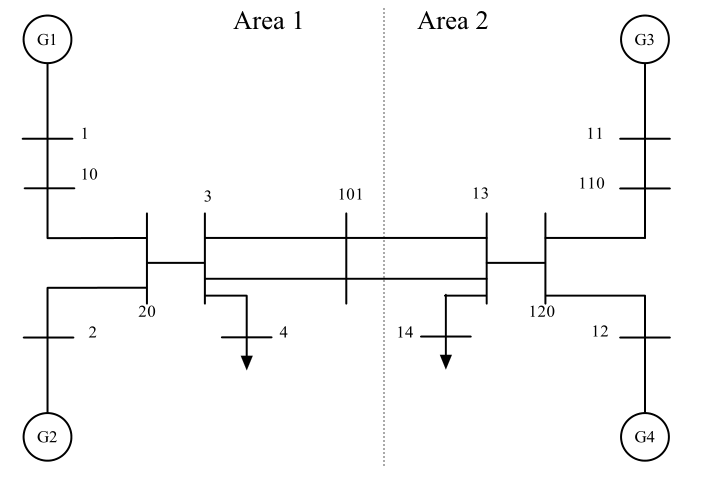
\includegraphics[width=\linewidth]{sysOneLineAreas}
\end{minipage}% 


\paragraph{Result Summary:}
\begin{itemize}
\item Interchange adjustment seems to work correctly and is accounted for in AGC calculations.
\item The use of \verb|mAGC_sig| was tested as working using FTS or VTS.
\end{itemize}

\begin{minipage}{.5\linewidth}

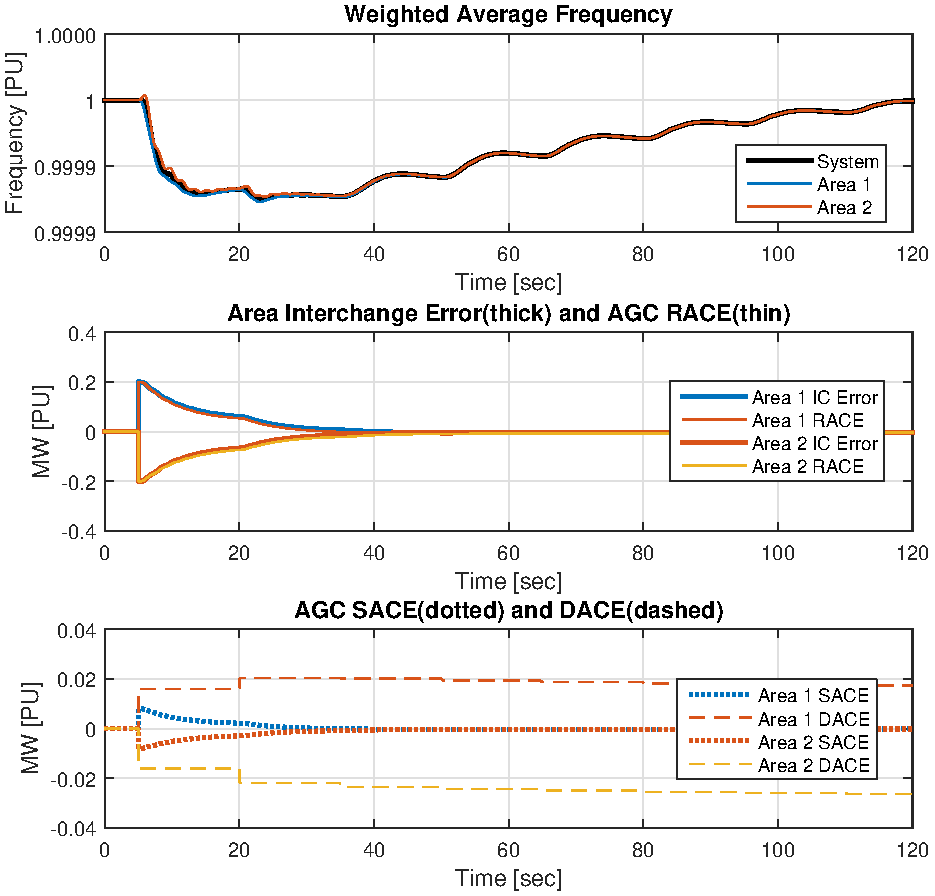
\includegraphics[width=\linewidth]{agcSigs}
\end{minipage}%
\begin{minipage}{.5\linewidth}

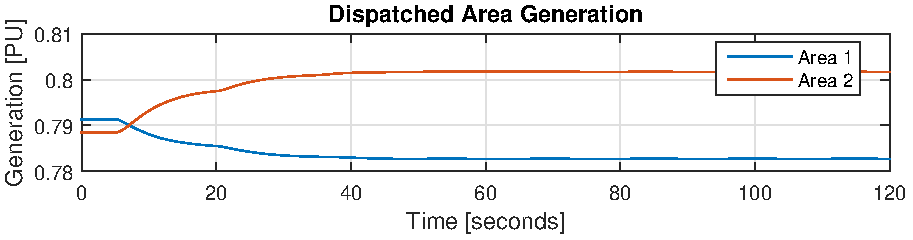
\includegraphics[width=\linewidth]{areaGen}

\vspace{1em}
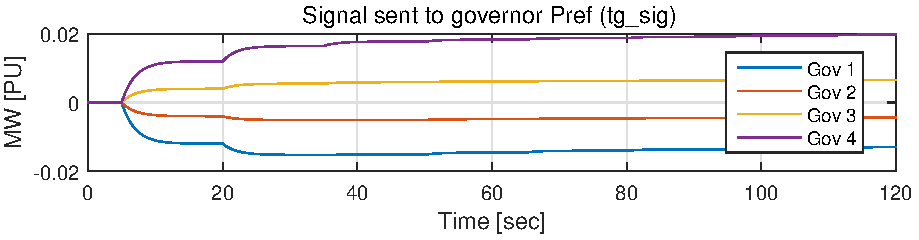
\includegraphics[width=\linewidth]{tgSigs}

\vspace{1em}
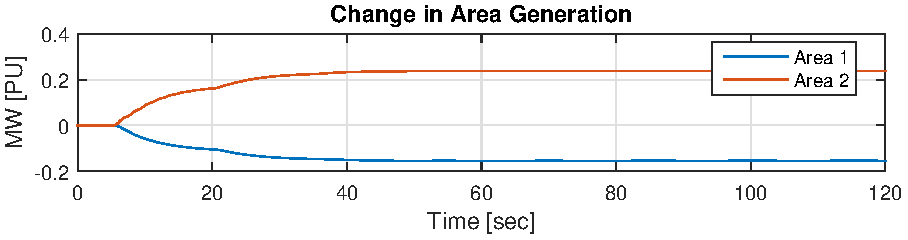
\includegraphics[width=\linewidth]{changeGen}
\end{minipage}

\paragraph{Why this might matter: } \ \\
An extended term simulation may required the adjustment of scheduled interchange to achieve system recovery.
Specifically, if an area realizes that their available reserves become lower than was originally allocated for, a resolution may be to import more power from another area.
This added functionality will allow custom logic to handle such a scenario.

\pagebreak
\paragraph{MATLAB modulation code} \ \\
The \verb|mAGC_sig| file that adjusts the interchange and forces AGC action is shown below.

\begin{minted}[
		frame=lines,
		framesep=2mm,
		baselinestretch=1.2,
		bgcolor=gray!13,
		fontsize=\footnotesize,
		linenos,
		breaklines
		]{MATLAB}
function mAGC_sig(k)
% Syntax: mAGC_sig(k)
% input k is current data index
% 09:46 08/21/20
% place to define modulation signal for AGC operation

global g

%{
    Scenario:
Area 1 is exporting generation to Area 2 (Interchange value Positive)
Area 2 is importing power from Area 1 (Interchange value is Negative

Area 2 increases scheduled interchage, which reduces its scheduled import and causes area 2 to increase generation.
Area 1 decreases scheduled interchange to balance area 2 action.
As area 1 is exporting, the negative valued icAdj will reduce the generation in the area.

%}
persistent ForceDisptach

if g.sys.t(k) >= 5
    % adjust iterchange 
    g.area.area(2).icAdj(k) = 0.2;
    g.area.area(1).icAdj(k) = -0.2;
    
    % force AGC disptatch when interchange adjustment first applied
    if ForceDisptach
        g.agc.agc(1).nextActionTime = g.sys.t(k);
        g.agc.agc(2).nextActionTime = g.sys.t(k);
        ForceDisptach = 0;
    end
    
else
    g.area.area(2).icAdj(k) = 0;
    g.area.area(1).icAdj(k) = 0;
    ForceDisptach = 1;
end
end
\end{minted}

\end{document}
